\subsection{Heun's Method}



\frame{
The next approach, Heun's method, introduces a new idea for constructing an algorithm to solve the I.V.P. 
\begin{equation}
y' (t) = f (t, y(t)) \ \ \ over \ \ \ [a, b] \ \ \ with \ \ y(t_0) = y_0
\end{equation}
%\begin{figure}
%\begin{center}
%\includegraphics[width=80mm]{fig/ch-6/eq_6-26.png}
%\end{center}
%\end{figure}
To obtain the solution point $(t_1, y_1)$, we can use the fundamental theorem of calculus and integrate $y'(t)$ over $[t_0, t_1]$ to get 
\begin{equation}
\int_{t_0}^{t_1} f (t, y(t)) d t = \int_{t_0}^{t_1} y'(t) dt = y(t_1) - y(t_0)
\end{equation}
%\begin{figure}
%\begin{center}
%\includegraphics[width=80mm]{fig/ch-6/eq_6-27.png}
%\end{center}
%\end{figure}
where the antiderivative of $y'(t$) is the desired function $y(t)$. 
When equation (6.27) is solved for $y(t_1)$, the result is
\begin{equation}
y(t_1) = y(t_0) + \int_{t_0}^{t_1} f (t, y(t)) dt
\end{equation}
%\begin{figure}
%\begin{center}
%\includegraphics[width=80mm]{fig/ch-6/eq_6-28.png}
%\end{center}
%\end{figure}
}

\frame{
Now a numerical integration method can be used to approximate the definite integral in (6.28). 
If the trapezoidal rule is used with the step size $h = t_1 - t_0$, then the result is 
\begin{equation}
y(t_1) \approx y(t_0) + \frac{h}{2} ( f (t_0, y(t_0)) + f (t_1, y(t_1))). 
\end{equation}
%\begin{figure}
%\begin{center}
%\includegraphics[width=80mm]{fig/ch-6/eq_6-29.png}
%\end{center}
%\end{figure}
Notice that the formula on the right-hand side of (6.29) involves the yet to be determined value $y(t_1)$. 
To proceed, we use an estimate for $y(t_1)$.
Euler's solution will suffice for this purpose. 
After it is substituted into (6.29), the resulting formula for finding $(t_1, y_1)$ is called {\Large Heun's method}: 
\begin{equation}
y_1 = y(t_0)+ \frac{h}{2} (f(t_0,y_0)+ f(t_1,y_0 +hf(t_0,y_0))). 
\end{equation}
%\begin{figure}
%\begin{center}
%\includegraphics[width=100mm]{fig/ch-6/eq_6-30.png}
%\end{center}
%\end{figure}
}

\frame{
\begin{itemize}
\item The process is repeated and generates a sequence of points that approximates the solution curve $y = y(t)$. 
\item At each step, Euler's method is used as a prediction, and then the trapezoidal rule is used to make a correction to obtain the final value. 
The general step for Heun's method is 
\end{itemize}
\begin{equation}
\begin{array}{l}
p_{k+1} = y_k + hf(t_k,y_k),	t_{k+1} = t_k + h, \\ 
\\
y_{k+1} = y_k + h(f(t_k,y_k) + f(t_{k+1},p_{k+1})).
\end{array}
\end{equation}
%\begin{figure}
%\begin{center}
%\includegraphics[width=100mm]{fig/ch-6/eq_6-31.png}
%\end{center}
%\end{figure}
}

\frame{
\begin{itemize}
\item Notice the role played by differentiation and integration in Heun's method. 
\item Draw the line tangent to the solution curve $y = y(t)$ at the point $(t_0, y_0)$ and use it to find the predicted point $(t_1,p_1)$. 
\item Now look at the graph $z = f(t,y(t))$ and consider the points $(t_0, f_0)$ and $(t_1, f_1)$, where $f_0 = f(t_0, y_0)$ and $f_1 = f(t_1,p_1)$. 
\item The area of the trapezoid with vertices $(t_0, f_0)$ and $(t_1, f_1)$ is an approximation to the integral in (6.28), which is used to obtain the final value in equation (6.30). 
\end{itemize}
}

\frame{
%The graphs are shown in Figure 6.7. 
\begin{figure}
\begin{center}
%\includegraphics[width=110mm]{fig/ch-6/fig_6-7.png}
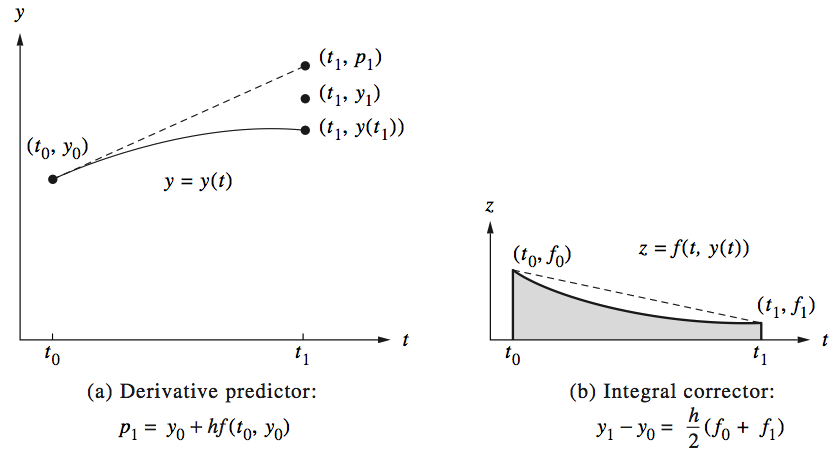
\includegraphics[width=110mm]{chap-6/fig_9-7.png}
\end{center}
\end{figure}
}

\frame{
\frametitle{Step Size versus Error}
The error term for the trapezoidal rule used to approximate the integral in (6.28) is
\begin{equation}
y''(c_k) \frac{h^3}{12}
\end{equation}
%\begin{figure}
%\begin{center}
%\includegraphics[width=60mm]{fig/ch-6/eq_6-32.png}
%\end{center}
%\end{figure}
If the only error at each step is that given in (6.32), after $M$ steps the accumulated error for Heun's method would be 
\begin{equation}
- \sum_{k =1}^M y''(c_k) \frac{h^3}{12} = \approx \frac{b-a}{12} y^{(2)}(c) h^2 = o(h^2)
\end{equation}
%\begin{figure}
%begin{center}
%\includegraphics[width=60mm]{fig/ch-6/eq_6-33.png}
%\end{center}
%\end{figure}
The next theorem is important, because it states the relationship between F.G.E. and step size. 
It is used to give us an idea of how much computing effort must be done to obtain an accurate approximation using Heun's method. 
}

\frame{
\begin{block}{Theorem 6.4 (Precision of Heun’s Method).}
Assume that $y(t)$ is the solution to the I.V.P. (1). 
If $y(t) \in C^3[t_0,b]$ and $\{ (t_k, y_k)\}_{k=0}^M$ is the sequence of approximations generated by Heun’s method, then
\begin{equation}
\begin{array}{r l}
\left| e_k \right|       & = \left| y(t_k) - y_k \right| = O(h^2) \ \
\\
\left| e_{k+1} \right| & = \left|  y(t_{k+1)} - y_k - h \Phi (t_k, y_k) \right|  = O(h^2) \\
\end{array}
\end{equation}
where
\begin{equation}
\Phi(t_k,y_k)= y_k +(h\slash2)(f(t_k,y_k)+ f(t_{k+1},y_k + hf(t_k,y_k)))
\end{equation}
\end{block}                                                                                                                                                                                                                                                                                                                                                                                                             
%\begin{figure}
%\begin{center}
%\includegraphics[width=110mm]{fig/ch-6/theorem_6-4.png}
%\end{center}
%\end{figure}
In particular, the final global error (F.G.E.) at the end of the interval will satisfy
\begin{equation}
E(y(b),h) = \left| y(b)-y_M\right|= O(h^2).
\end{equation}
%\begin{figure}
%\begin{center}
%\includegraphics[width=70mm]{fig/ch-6/eq_6-35.png}
%\end{center}
%\end{figure}
}

\frame{
Examples 6.6 and 6.7 illustrate Theorem 6.4. 
If approximations are computed using the step sizes hand $h/2$, we should have 
\begin{equation}
E(y(b), h) \approx C h^2
\end{equation}
%\begin{figure}
%\begin{center}
%\includegraphics[width=70mm]{fig/ch-6/eq_6-36.png}
%\end{center}
%\end{figure}
for the larger step size, and 
\begin{equation}
E \left( y(b), \frac{h}{2} \right) \approx C \frac{h^2}{4} = \frac{1}{4} C h^2 \approx \frac{1}{4} E(y(b),h)
\end{equation}
%\begin{figure}
%\begin{center}
%\includegraphics[width=90mm]{fig/ch-6/eq_6-37.png}
%\end{center}
%\end{figure}
Hence the idea in Theorem 6.4 is that if the step size in Heun's method is reduced by a factor of $\frac{1}{2}$ we can expect that the overall F.G.E. will be reduced by a factor of $\frac{1}{4}$· 
}

\frame{
\begin{block}{Example 6.6.}
Use Heun’s method to solve the I.V.P.
\begin{equation}
y' = \frac{t-y}{2} \ \ \ \ \ on \ \ \ [0,3] \ \ with \ \ y(0) = 1
\end{equation}
Compare solutions for $h = 1$, $\frac{1}{2}$ ,$\frac{1}{4}$, and $\frac{1}{8}$.
\end{block}
%\begin{figure}
%\begin{center}
%\includegraphics[width=110mm]{fig/ch-6/ex_6-6.png}
%\end{center}
%\end{figure}
Figure 6.8 shows the graphs of the first two Heun solutions and the exact solution curve $y(t) = 3e^{-t/2} - 2 + t$. 
Table 6.4 gives the values for the four solutions at selected abscissas. 
}

\frame{
For the step size $h = 0.25$, a sample calculation is 
\begin{equation}
\begin{array}{r l}
f(t_0, y_0) & = \frac{0-1}{2} = -0.5 \\
& \\
p_1 & = 1.0 + 0.25(-0.5) = 0.875 \\
& \\
f(t_1,p_1) & = \frac{0.25-0.875}{2} = -0.3125 \\
& \\
y_1 & = 1.0 + 0.125(-0.5 - 0.3125) = 0.8984375
\end{array}
\end{equation}
%\begin{figure}
%\begin{center}
%\includegraphics[width=80mm]{fig/ch-6/p_263.png}
%\end{center}
%\end{figure}
This iteration continues until we arrive at the last step: 
\begin{equation}
y(3) \approx y_12 = 1.511508 + 0.125(0.619246 + 0.666840) = 1.672269.
\end{equation}
%\begin{figure}
%\begin{center}
%\includegraphics[width=100mm]{fig/ch-6/p_263_2.png}
%\end{center}
%\end{figure}
}

\frame{
\begin{figure}
\begin{center}
%\includegraphics[width=90mm]{fig/ch-6/fig_6-8.png}
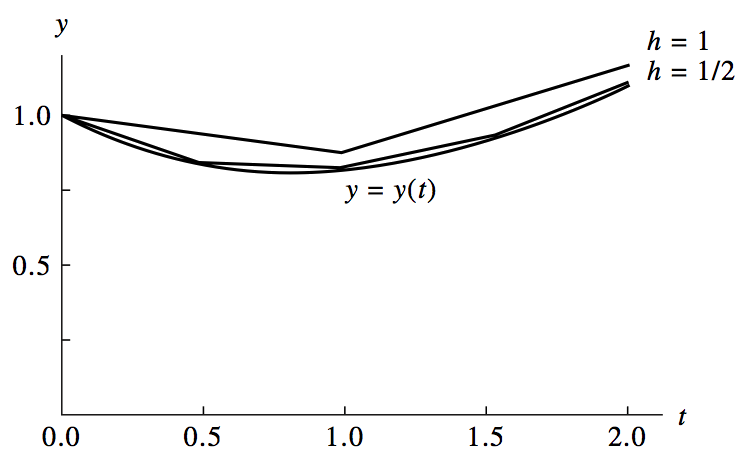
\includegraphics[width=60mm]{chap-6/fig_9-8.png}
\end{center}
\end{figure}
%}
%\frame{
\begin{figure}
\begin{center}
%\includegraphics[width=80mm]{fig/ch-6/tab_6-4.png}
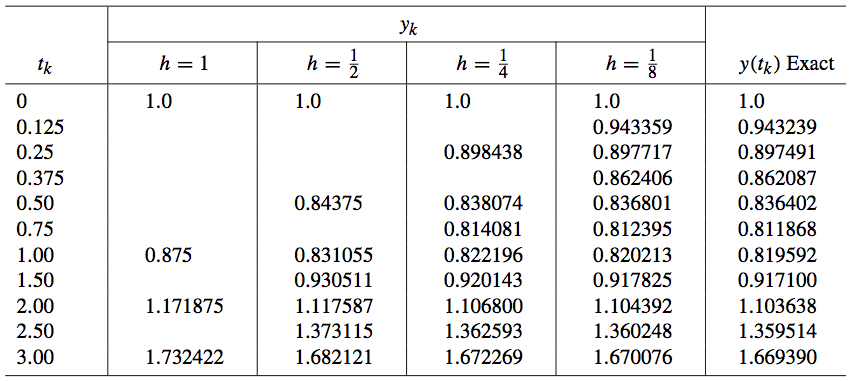
\includegraphics[width=80mm]{chap-6/tab_9-4.png}
\end{center}
\end{figure}
}

\frame{
\begin{block}{Example 6.7.}
Compare the F.G.E. when Heun’s method is used to solve
\begin{equation}
y' = \frac{t-y}{2} \ \ \ \ \ over \ \ \ [0,3] \ \ \ with \ \ y(0) = 1
\end{equation}
using step sizes $1$, $\frac{1}{2}$, $\ldots$, $\frac{1}{64}$
\end{block}
Table 6.5 gives the F.G.E. and shows that the error in the approximation to $y(3)$ decreases by about $\frac{1}{4}$ when the step size is reduced by a factor of $\frac{1}{2}$ :
\begin{equation}
E(y(3), h) = y(3) - y_M = O(h^2) \approx Ch^2, \ \ \ where C = -0.0432.
\end{equation}
%\begin{figure}
%\begin{center}
%\includegraphics[width=110mm]{fig/ch-6/ex_6-7.png}
%\end{center}
%\end{figure}
}

\frame{
\begin{figure}
\begin{center}
%\includegraphics[width=80mm]{fig/ch-6/tab_6-5.png}
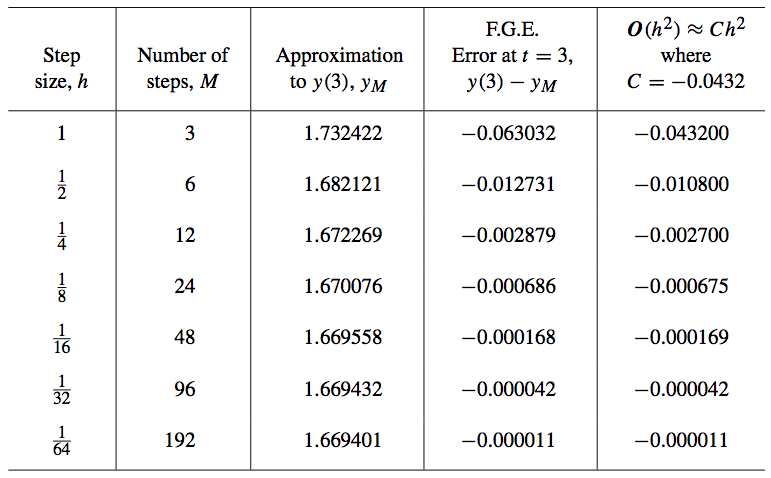
\includegraphics[width=80mm]{chap-6/tab_9-5.png}
\end{center}
\end{figure}
}

%\frame{
%\begin{figure}
%\begin{center}
%\includegraphics[width=110mm]{fig/ch-6/prog_6-2.png}
%\end{center}
%\end{figure}
%}


